\section{Motivation de l'étude}

Les travaux de \cite{romain25} s'inscrivent dans une approche de calcul à zones couplant conduction et rayonnement, où chaque surface est caractérisée par une unique température moyenne. Cette approche, bien qu'efficace, ne permet pas de rendre compte des écarts de température au sein d'une même surface, écarts pourtant susceptibles d'être significatifs dans des configurations à forte hétérogénéité de puissance.

Cette étude se place dans une perspective différente et complémentaire : il ne s'agit plus de raffiner un modèle à zones, mais d'exploiter directement les capacités de la simulation CFD 3D pour accéder, en plus de la température moyenne $T_{\mathrm{moy}}$, aux températures extrémales $T_{\mathrm{max}}$ et $T_{\mathrm{min}}$ d'une géométrie représentative d'un assemblage de crayons combustible. L'objectif de ce chapitre est ainsi de \textbf{démontrer la faisabilité d'une étude 3D exigeante}, \textbf{de quantifier le biais de convergence} de la disctétisation des faces radiatives introduit par les hypothèses du modèle rayonnement en milieu transparent et d'étudier \textbf{l'écart entre le point chaud de  l'assemblage et sa température moyenne}.


\section{Mise en place numérique}

\subsection{Description de la configuration étudiée}

La configuration étudiée est représentative d'un assemblage de crayons combustible, organisé selon un réseau carré de $5\times5$ crayons. Les paramètres géométriques de cet assemblage sont résumés dans le Tableau~\ref{tab:geom_assemblage}, et le domaine de calcul est illustré à la Figure~\ref{fig:domaine}.

\begin{table}[H]
\centering
\renewcommand{\arraystretch}{1.0}
\begin{tabular}{lcc}
\toprule
Paramètre & Symbole & Valeur \\
\midrule
Nombre de crayons (réseau $5\times5$) & $N_{\mathrm{pins}}$ & $25$ \\
Pas du réseau (centre à centre)& $p$ & $16{,}26$~mm \\
Rayon d'un crayon & $R$ & $6{,}26$~mm \\
Hauteur active d'un crayon & $H$ & $250{,}4$~mm \\
\bottomrule
\end{tabular}
\caption{Paramètres géométriques de l'assemblage de crayons combustible.}
\label{tab:geom_assemblage}
\end{table}

\begin{figure}[H]
\centering
\begin{minipage}{0.45\textwidth}
    \centering
    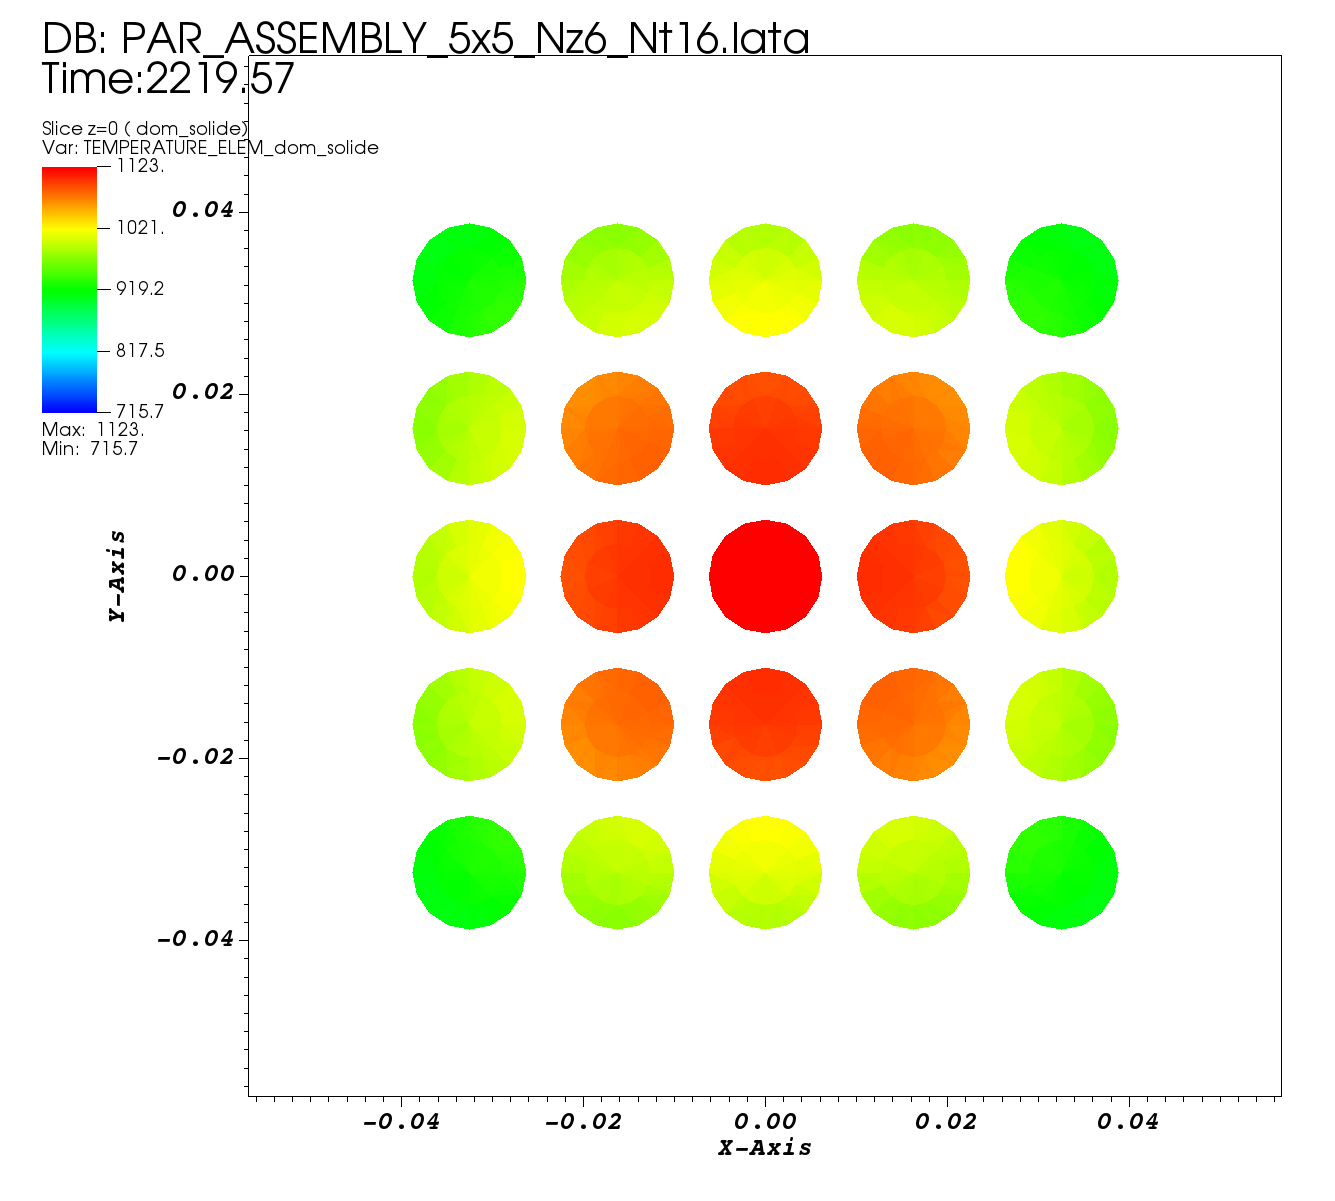
\includegraphics[width=\linewidth]{PICTURES/c5couplage/slicez0.png}
\end{minipage}
\hfill
\begin{minipage}{0.45\textwidth}
    \centering
    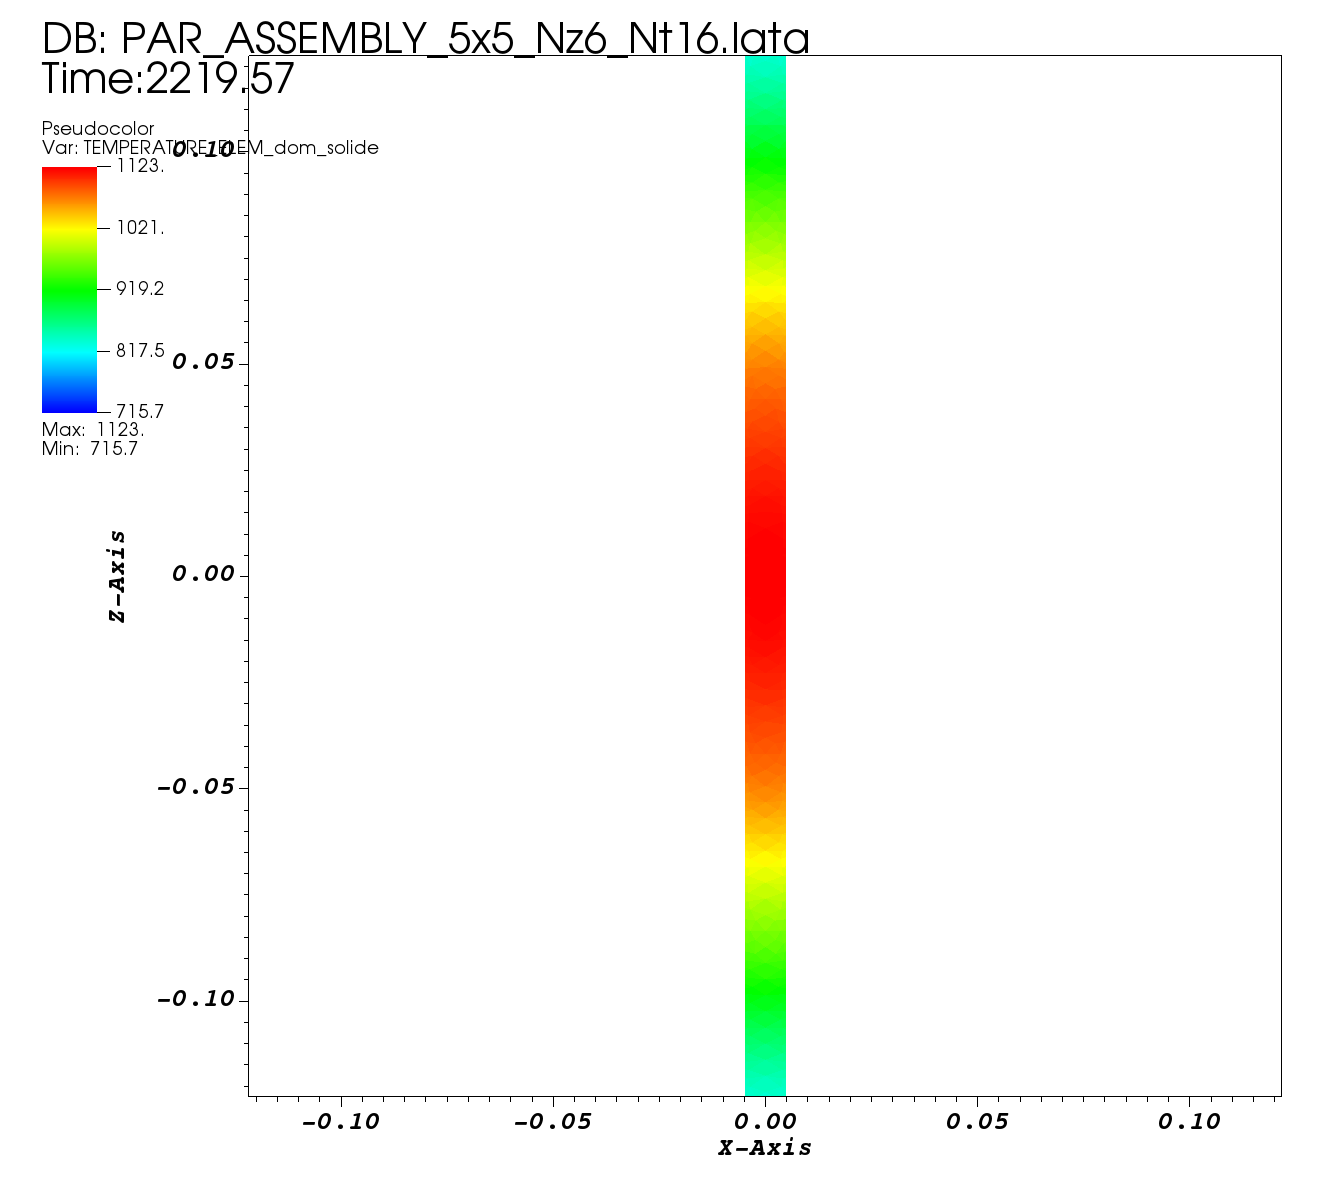
\includegraphics[width=\linewidth]{PICTURES/c5couplage/sliceMid.png}
\end{minipage}
\caption{Plan de coupe en $Z=0$ (gauche) et coupe verticale du crayon central (droite).}
\label{fig:domaine}
\end{figure}

Le combustible et le fluide caloporteur sont caractérisés par les propriétés thermophysiques et radiatives résumées dans le Tableau~\ref{tab:proprietes}. Plusieurs niveaux de puissance volumique sont déposés dans le combustible, modulés selon un profil axial en cosinus caractéristique de la distribution de puissance neutronique le long d'un crayon combustible ; aucune source de puissance n'est imposée dans le fluide. Ces cas correspondent à des températures moyennes croissantes du crayon central, permettant d'étudier l'effet de la discrétisation sur une gamme de régimes thermiques représentative. Le fluide est par ailleurs traité sous l'hypothèse de Boussinesq, avec une gravité orientée selon $-\vec{z}$. Une température de paroi $T_{\mathrm{paroi}} = 600$~K est imposée en périphérie du domaine.

\begin{table}[H]
\centering
\begin{tabular}{lccc}
\toprule
Propriété & Symbole & Combustible & Fluide \\
\midrule
Masse volumique & $\rho$~[$\mathrm{kg/m^3}$] & $10\,110$ & $6{,}754\times10^{-5}$ \\
Conductivité thermique & $\lambda$~[$\mathrm{W/(m.K)}$] & $10$ & $0{,}01$ \\
Capacité calorifique & $C_p$~[$\mathrm{J/(kg.K)}$] & $350$ & $1141{,}1$ \\
Viscosité dynamique & $\mu$~[$\mathrm{Pa.s}$] & -- & $4{,}153\times10^{-5}$ \\
Coefficient de dilatation thermique & $\beta_{\mathrm{th}}$~[$\mathrm{K^{-1}}$] & -- & $10^{-3}$ \\
Émissivité & $\epsilon$ & $1$ & -- \\
\bottomrule
\end{tabular}
\caption{Propriétés thermophysiques et radiatives du combustible et du fluide caloporteur.}
\label{tab:proprietes}
\end{table}

\subsection{Maillage}

Le maillage surfacique des crayons est généré à l'aide de l'algorithme \texttt{MG-CADSurf} de la plateforme \textsc{Salome}, avec une taille de maille cible comprise entre $2$~mm et $10$~mm ; la section circulaire de chaque crayon y est approximée par un polygone à $N_\theta = 16$ côtés, valeur maximale de discrétisation radiale atteignable compte tenu des limitations des outils de simulation utilisés. Ce maillage de surface constitue le support du calcul des facteurs de vue par lancer de rayons, et offre une bonne approximation de la géométrie cylindrique. Le maillage volumique du domaine fluide, nécessaire à la résolution du problème thermohydraulique dans \textsc{Trust}, est ensuite généré à partir de ce maillage surfacique à l'aide de l'algorithme tétraédrique \texttt{MG-Tetra}, et comporte environ $1{,}2$ million d'éléments. La Figure~\ref{fig:mesh} présente une coupe horizontale et une coupe verticale de ce maillage.

\begin{figure}[H]
\centering
\begin{minipage}{0.45\textwidth}
    \centering
    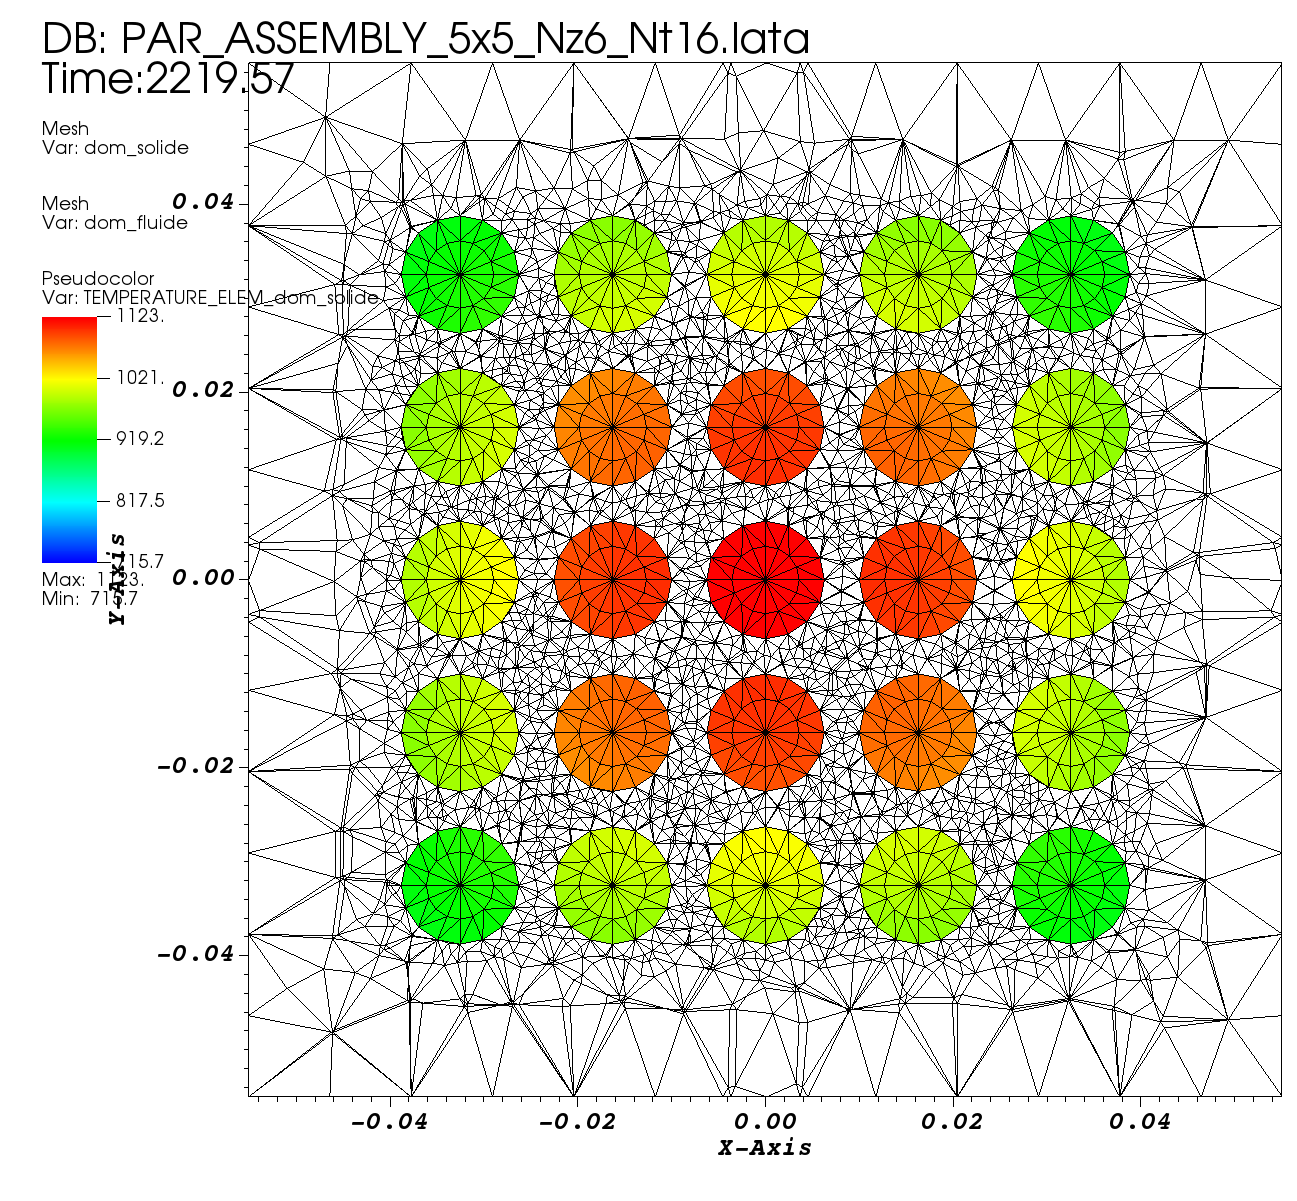
\includegraphics[width=\linewidth]{PICTURES/c5couplage/mesh_horizontal.png}
\end{minipage}
\hfill
\begin{minipage}{0.45\textwidth}
    \centering
    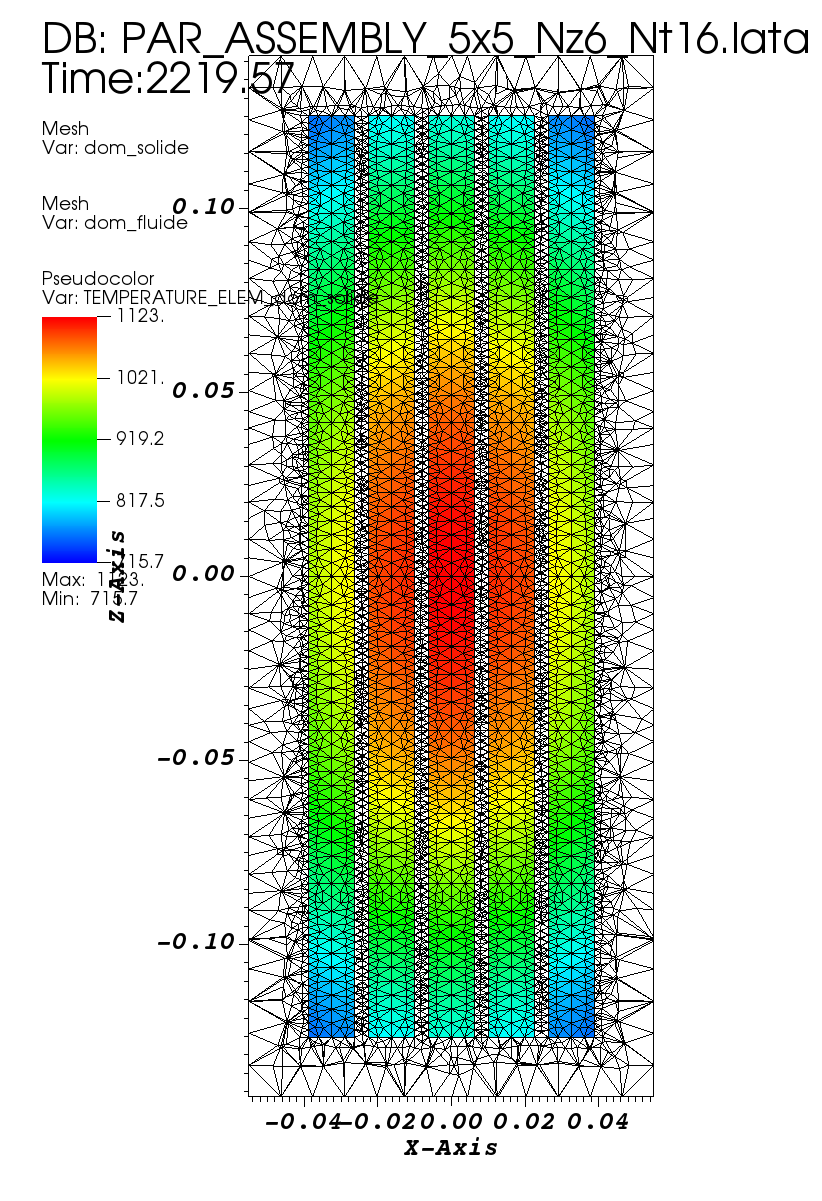
\includegraphics[width=\linewidth]{PICTURES/c5couplage/mesh_vertical.png}
\end{minipage}
\caption{Coupe horizontale en $Z=0$ (gauche) et coupe verticale (droite) du maillage volumique.}
\label{fig:mesh}
\end{figure}

\subsection{Discrétisation des faces radiatives}

Cette étude se concentre sur l'effet du raffinement axial de la discrétisation radiative, la sensibilité à la discrétisation radiale ayant déjà été étudiée en 2D par \cite{romain25}. La surface de chaque crayon est ainsi découpée, pour les besoins du calcul radiatif, en $N_\theta \times N_z$ sous-surfaces élémentaires, chacune résultant du croisement d'un secteur angulaire, hérité des $N_\theta = 16$ faces planes du maillage géométrique, avec une tranche axiale parmi les $N_z$ retenues. Le nombre de secteurs angulaires $N_\theta = 16$, fixé par des limitations des outils \salome et \trust, reste ainsi constant pour l'ensemble de cette étude. Seul le nombre de tranches axiales $N_z$ — paramètre propre à la discrétisation radiative, indépendant du maillage volumique — est varié, sur la plage $2, 4, \dots, 20$, afin de quantifier le biais introduit par l'hypothèse de radiosité uniforme au sein de chaque sous-surface.


\subsection{Stratégie de résolution numérique}

Le problème thermohydraulique couplé est résolu dans \textsc{Trust} par une méthode de volumes finis. Bien que l'objectif de cette étude soit d'obtenir l'état stationnaire du système, \textsc{Trust} résout ce problème par une approche de marche en temps : le schéma numérique fait converger la solution vers un point fixe stationnaire par intégration temporelle successive.

Le schéma retenu est un schéma d'Euler implicite, dont le pas de temps $\mathrm{d}t$ est piloté automatiquement entre les bornes $\mathrm{d}t_{\mathrm{min}}$ et $\mathrm{d}t_{\mathrm{max}}$ par un facteur de sécurité \texttt{facsec}. Ce facteur ajuste le pas de temps à chaque itération en fonction de la vitesse de convergence du solveur implicite, permettant d'accélérer la marche en temps tant que la convergence du système linéaire reste satisfaisante. Les principaux paramètres du schéma sont résumés en Annexe~ref{tab:solveur}.

La valeur de \texttt{facsec} retenue, très supérieure à l'unité, illustre bien la nature de cette stratégie : le pas de temps n'est plus piloté par un critère de précision physique de la dynamique transitoire, mais uniquement par la vitesse à laquelle le solveur implicite parvient à converger à chaque itération. Cette approche revient ainsi à utiliser l'intégration temporelle comme un simple outil numérique permettant d'atteindre efficacement l'état stationnaire recherché, sans chercher à représenter fidèlement une éventuelle dynamique transitoire réelle du système. Le calcul est considéré comme convergé lorsque l'évolution de la solution entre deux pas de temps successifs devient inférieure au seuil de stationnarité \texttt{seuil\_statio}.


\section{Résultats}

\subsection{Vérifications préliminaires}

Avant d'exploiter les résultats de température issus des simulations, deux vérifications préliminaires ont été menées afin de s'assurer de la cohérence physique du montage numérique.

La première concerne le profil de puissance imposé dans le combustible. La puissance volumique déposée devant suivre un profil axial en cosinus, représentatif de la distribution de puissance neutronique le long d'un crayon, le profil de température obtenu au centre du crayon central (Figure~\ref{fig:profil}) est comparé à ce profil attendu et montre une bonne adéquation avec les résultats de la simulation.

\begin{figure}[H]
\centering
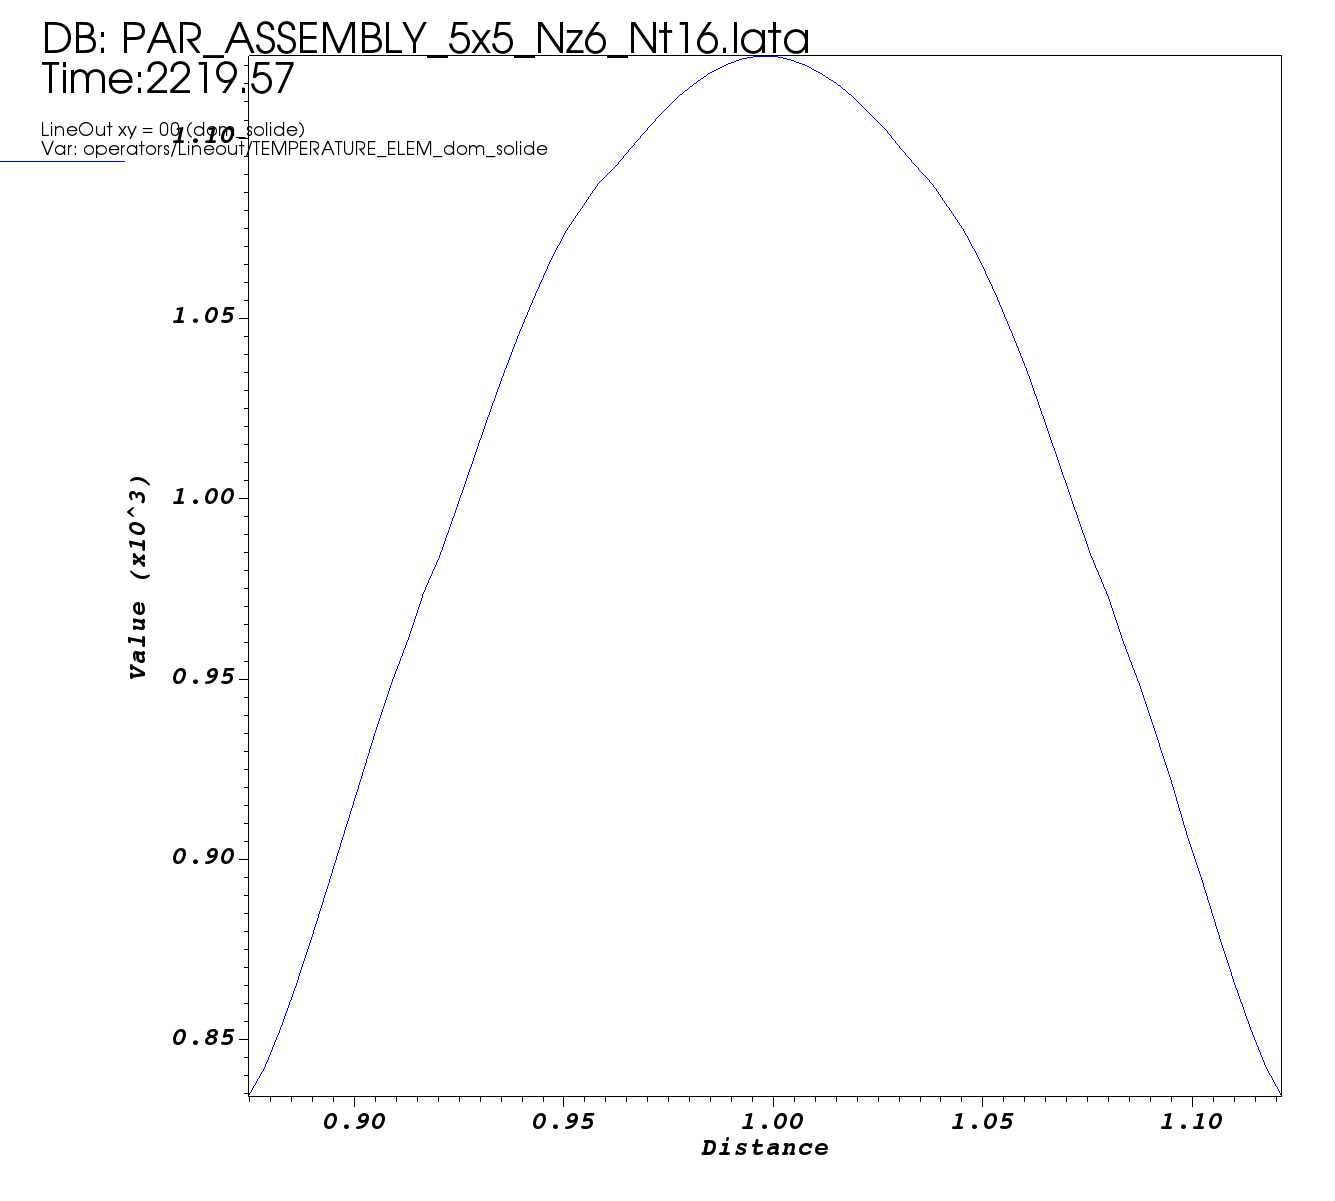
\includegraphics[width=0.4\linewidth]{PICTURES/c5couplage/lineout.png}
\caption{Profil axial de température au centre du crayon central.}
\label{fig:profil}
\end{figure}

La seconde vérification porte sur la conservation globale de l'énergie au sein du système. En régime stationnaire, la puissance totale déposée dans le combustible doit être intégralement évacuée par les mécanismes de transfert thermique du domaine, à savoir le rayonnement et la diffusion thermique à travers les parois du domaine. Le bilan global de puissance s'écrit ainsi :

\begin{equation}
    P_{\mathrm{déposée}} = P_{\mathrm{sortante}}, \qquad \text{avec } P_{\mathrm{sortante}} = P_{\mathrm{rad}} + P_{\mathrm{diffusion}},
    \label{eq:bilan_puissance}
\end{equation}

où $P_{\mathrm{déposée}}$ désigne la puissance volumique totale injectée dans le combustible, $P_{\mathrm{rad}}$ la puissance évacuée par rayonnement et $P_{\mathrm{diffusion}}$ celle évacuée par diffusion thermique à travers les parois du domaine. Cette égalité a été vérifiée sur l'ensemble des cas étudiés, avec un écart relatif compris entre quelques dizaines de pcm et $1\,\%$ selon les cas, confirmant, même dans la configuration la moins favorable, la cohérence du bilan thermique global de la simulation.


\subsection{Sensibilité à la discrétisation axiale}
\label{sec:consequence_radiosite}

La sensibilité de la solution thermique à la discrétisation axiale est étudiée pour trois niveaux de puissance représentatifs : $3$, $4$ et $45~\mathrm{MW/m^3}$, correspondant respectivement à des températures moyennes du crayon central d'environ $925$~K, $980$~K et $1817$~K. Le paramètre $N_z$ désigne le nombre de découpes selon l'axe $z$ des crayons; il ne s'agit pas d'un raffinement du maillage au sens numérique du terme, mais d'une discrétisation de la représentation des propriétés thermiques et radiatives, chaque sous-géométrie se voyant associer une température uniforme servant de température effective dans le calcul des échanges radiatifs.

Cette distinction est essentielle dans le cas étudié, où la puissance volumique suit un profil axial en cosinus, maximal au centre du domaine actif (Figure~\ref{fig:profil}). Une faible valeur de $N_z$ revient à homogénéiser thermiquement des portions axiales étendues du champ de température, tandis qu'une valeur élevée permet de résoudre les variations axiales locales. L'objectif de cette section est de quantifier l'influence de cette discrétisation sur les échanges radiatifs et sur le champ de température résultant.

Pour chaque niveau de puissance, les températures minimale, maximale et moyenne sont comparées à la solution de référence obtenue pour $N_z=20$, à partir de l'écart relatif

\begin{equation}
\varepsilon_T(N_z)
=
\frac{\left|T(N_z)-T(N_z=20)\right|}
{T(N_z=20)}.
\end{equation}

Avant d'analyser les résultats, il est utile de préciser l'origine physique de l'erreur introduite par cette représentation. Le flux surfacique net émis par rayonnement obéit, d'après l'Équation~\eqref{eq:nice_qr}, à \ref{def:radio}. Le caractère convexe de la fonction $T \mapsto T^4$ implique, d'après l'inégalité de Jensen, que pour toute distribution de température non uniforme discrétisée en $M$ éléments de surface égale au sein d'une sous-géométrie,

\begin{equation}
\overline{T^4}
=
\frac{1}{M}\sum_{k=1}^{M} T_k^4
\;>\;
\overline{T}^{\,4},
\qquad
\overline{T} = \frac{1}{M}\sum_{k=1}^{M} T_k,
\label{eq:jensen}
\end{equation}

l'égalité n'étant atteinte que pour un champ uniforme ($T_k$ identique $\forall k$).

\subsubsection{Cas $\overline{T} \approx 925{,}7~\mathrm{K}$}

La Figure~\ref{fig:temperature3MW} compare les champs de température obtenus avec $N_z=4$ et $N_z=20$, ainsi que leur différence. La Figure~\ref{fig:convergence3MW} présente l'évolution, en fonction de $N_z$, des écarts relatifs des températures minimale, maximale et moyenne par rapport à la solution de référence.

\begin{figure}[H]
\centering
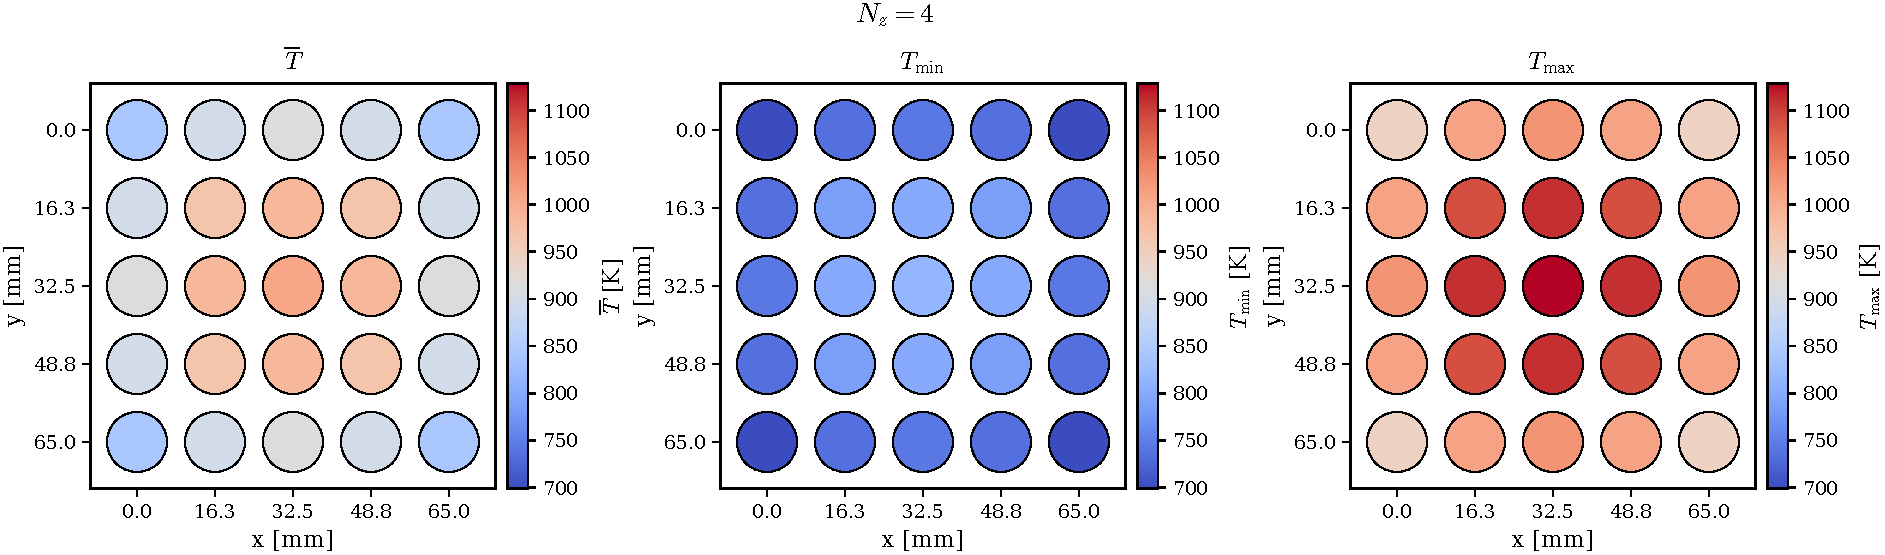
\includegraphics[width=0.8\linewidth]{PICTURES/c5couplage/T925/assembly_4.pdf}

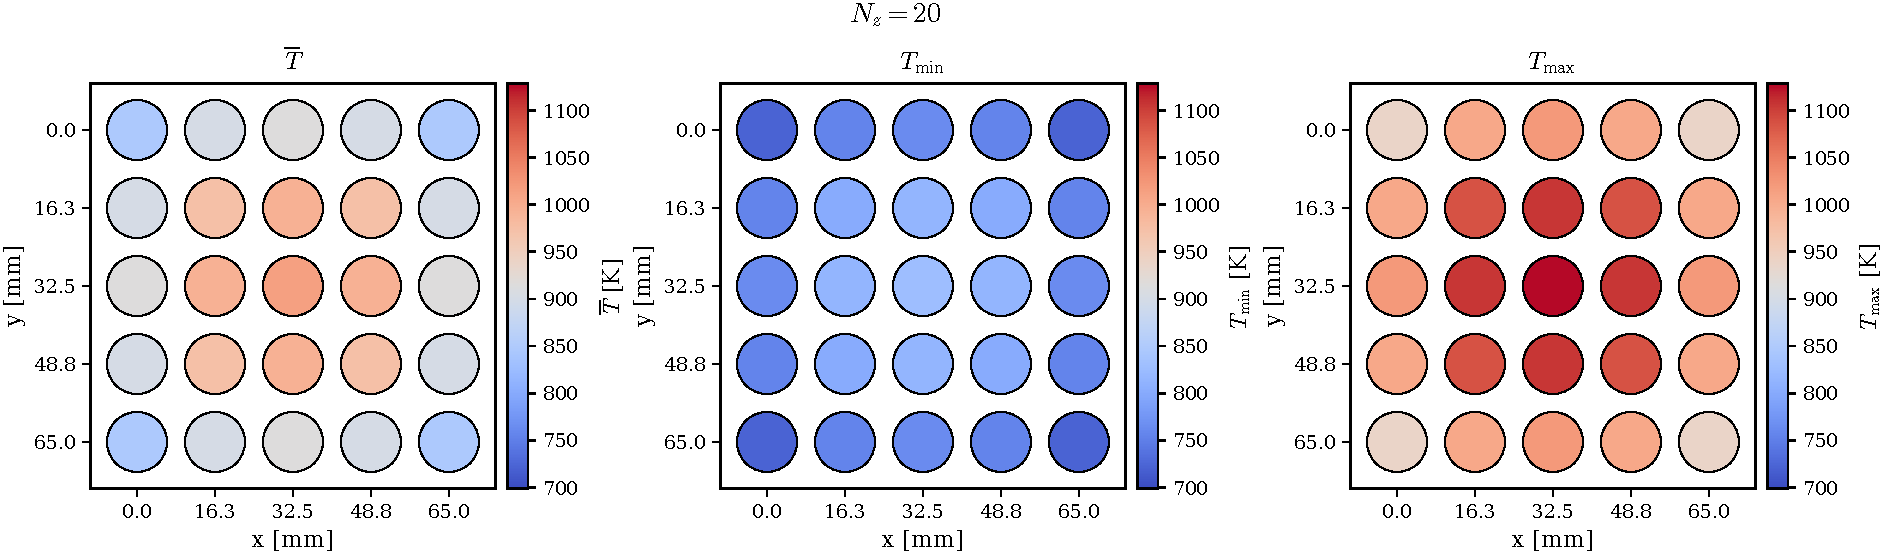
\includegraphics[width=0.8\linewidth]{PICTURES/c5couplage/T925/assembly_20.pdf}

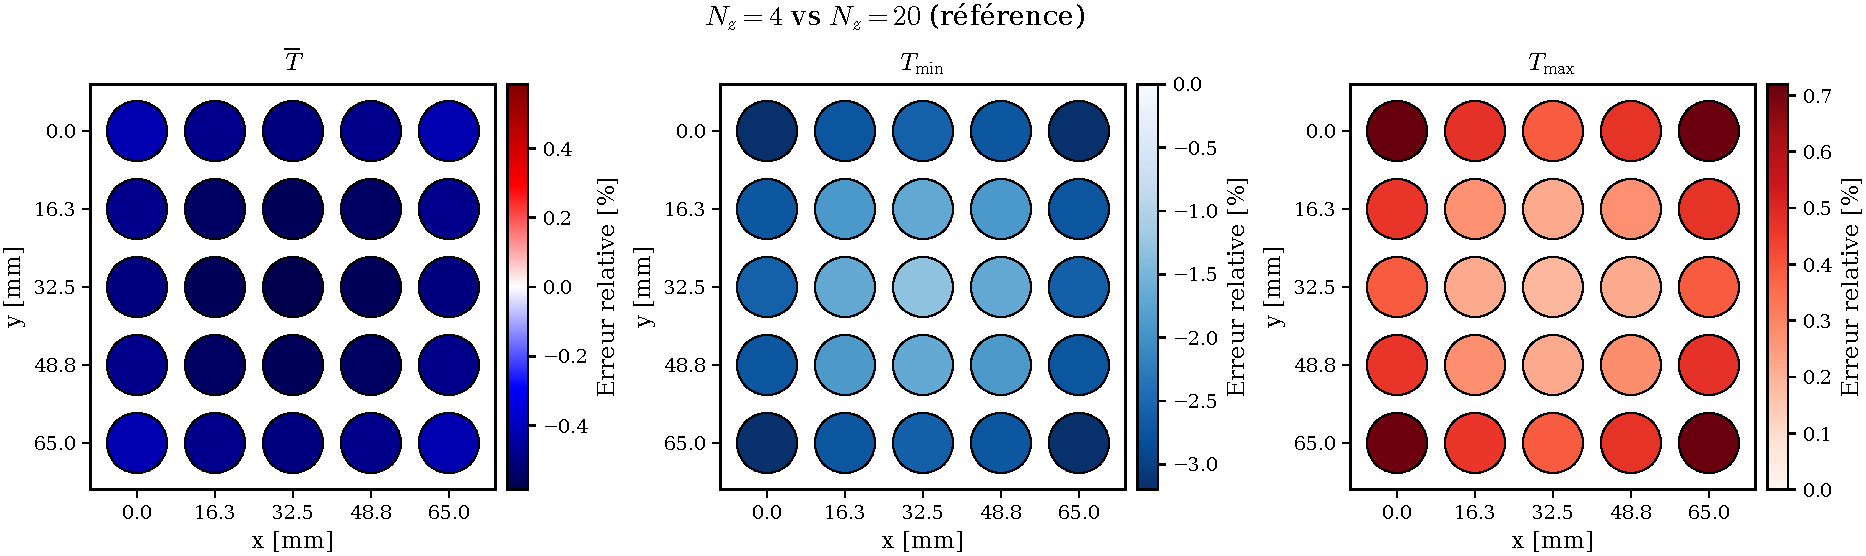
\includegraphics[width=0.8\linewidth]{PICTURES/c5couplage/T925/assembly_diff_4_vs_20.pdf}
\caption{Champs de température pour $\overline{T}=925{,}7~\mathrm{K}$ : $N_z=4$ (haut), $N_z=20$ (milieu) et différence entre les deux champs (bas).}
\label{fig:temperature3MW}
\end{figure}

\begin{figure}[H]
\centering
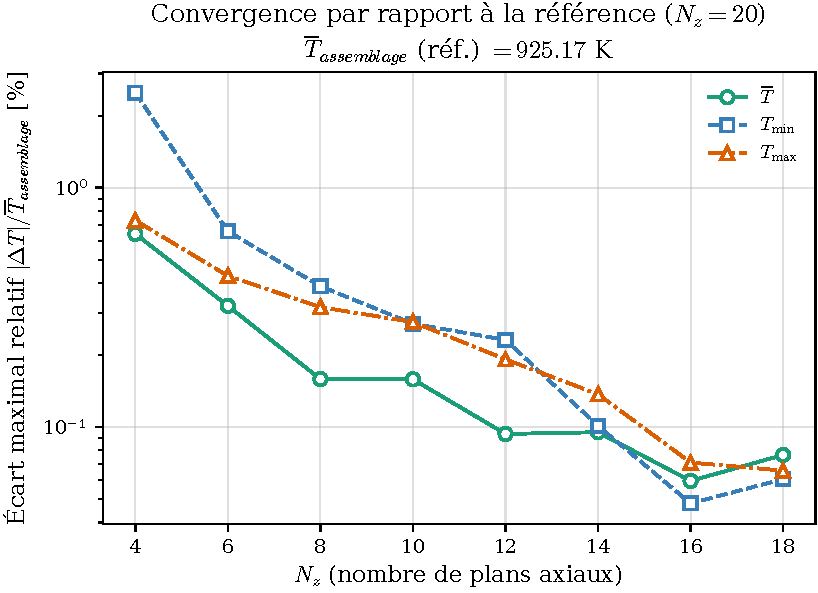
\includegraphics[width=0.7\linewidth]{PICTURES/c5couplage/T925/convergence_relative_vs_20.pdf}
\caption{Écart relatif des températures minimale, maximale et moyenne en fonction de $N_z$, par rapport à la référence $N_z=20$, pour $\overline{T}=925{,}7~\mathrm{K}$.}
\label{fig:convergence3MW}
\end{figure}

La Figure~\ref{fig:convergence3MW} met en évidence une convergence des trois grandeurs vers la solution de référence lorsque $N_z$ augmente : l'accroissement du raffinement axial permet de résoudre de plus en plus finement les variations thermiques axiales. Par exemple à partir de $N_z=14$, les écarts relatifs sont de l'ordre de $10^{-3}$, ce qui indique une bonne convergence du modèle.

Cette convergence s'interprète directement à la lumière de l'inégalité~\eqref{eq:jensen}. Dans chaque sous-géométrie, les propriétés radiatives sont évaluées à partir d'une température de surface uniforme. Une discrétisation axiale grossière assimile donc une portion étendue du profil thermique à une température unique, ce qui sous-estime la puissance rayonnée. Lorsque $N_z$ augmente, l'étendue axiale représentée par chaque température diminue, l'écart $\overline{T^4}-\overline{T}^{\,4}$ se réduit, et le bilan radiatif calculé tend vers celui du champ continu. Le raffinement axial ne constitue donc pas une simple amélioration: il détermine la fidélité avec laquelle le champ de température est \og vu \fg{} par le modèle radiatif.

La comparaison des champs de la Figure~\ref{fig:temperature3MW} montre par ailleurs que cette approximation ne modifie pas la structure thermique globale de l'assemblage : le crayon central demeure le plus chaud et les quatre crayons d'angle les plus froids, quelle que soit la valeur de $N_z$. Cette organisation spatiale est imposée par la géométrie de l'assemblage et par la configuration des échanges entre surfaces. La discrétisation axiale ne fait donc que moduler localement les niveaux de température, sans remettre en cause la hiérarchie thermique entre les crayons.

Les écarts sont en revanche nettement plus marqués sur les températures extrêmes que sur la température moyenne. Aux faibles valeurs de $N_z$, $T_{\max}$ est surestimée d'au plus $0{,}7\,\%$, tandis que $T_{\min}$ et $\overline{T}$ sont sous-estimées respectivement jusqu'à $3\,\%$ et $0{,}5\,\%$. Cette hiérarchie s'explique par la nature des grandeurs considérées : la température moyenne est une grandeur intégrée sur l'ensemble de l'assemblage, dans laquelle les erreurs locales de signes opposés se compensent partiellement, alors que $T_{\min}$ et $T_{\max}$ sont des grandeurs ponctuelles attachées aux régions les plus froides et les plus chaudes, précisément celles où les gradients --- et donc l'écart de l'inégalité~\eqref{eq:jensen} --- sont les plus importants.

Le signe de l'écart sur $T_{\max}$ s'interprète dans la région centrale, où le profil de puissance est maximal. Lorsque plusieurs positions axiales sont regroupées dans une même sous-géométrie, la température homogénéisée y est inférieure à la température réellement atteinte au point chaud. D'après l'inégalité~\eqref{eq:jensen}, la puissance radiative émise par cette sous-géométrie est alors sous-estimée : le puits radiatif est trop faible, et l'équilibre thermique local ne peut être rétabli qu'au prix d'une élévation de la température. Il en résulte une surestimation de $T_{\max}$ par rapport à la solution finement discrétisée.

Le comportement de $T_{\min}$ relève d'un mécanisme différent. La température des régions froides ne dépend pas seulement de leur propre émission : elle résulte du bilan entre la puissance radiative reçue des surfaces chaudes environnantes, leurs pertes radiatives et les transferts conductifs au sein de l'assemblage. La sous-estimation des émissions dans les zones chaudes voisines se propage donc, via le réseau des échanges radiatifs, jusqu'aux régions froides. L'écart observé sur $T_{\min}$ n'est ainsi pas la conséquence directe d'une moyenne locale, mais la signature du couplage entre la non-linéarité du rayonnement et la redistribution thermique à l'échelle de l'assemblage.

\begin{table}[H]
\centering
\caption{Écarts relatifs maximaux observés par rapport à la référence $N_z=20$ pour $\overline{T}=925{,}7~\mathrm{K}$.}
\label{tab:ecarts_discretisation_axiale}
\begin{tabular}{lcc}
\hline
Grandeur & Sens de l'écart & Écart maximal \\
\hline
$T_{\max}$ & Surestimation & $+0{,}7\,\%$ \\
$T_{\min}$ & Sous-estimation & $-3{,}0\,\%$ \\
$\overline{T}$ & Sous-estimation & $-0{,}5\,\%$ \\
\hline
\end{tabular}
\end{table}

Il convient enfin de s'assurer que ces écarts ne proviennent pas de la précision intrinsèque de la résolution numérique. Le critère de convergence du solveur thermique garantit une stabilisation de la température moyenne à environ $0{,}1~\mathrm{K}$, soit, pour $\overline{T}\approx925{,}7~\mathrm{K}$, une incertitude relative de
\begin{equation}
\frac{0{,}1}{925{,}7} \approx 1{,}1\times10^{-4}.
\end{equation}
Cette incertitude est inférieure d'au moins un ordre de grandeur aux écarts relatifs obtenus pour les discrétisations les plus grossières. Les différences observées entre les solutions sont donc bien attribuables à la discrétisation axiale et à son influence sur la représentation des échanges radiatifs, et non à une convergence insuffisante du solveur.

Pour ce niveau de puissance, un raffinement jusqu'à $N_z=14$ suffit ainsi à obtenir une représentation peu baisée la poursuite du raffinement devient peu pertinente, l'erreur de discrétisation étant déjà faible devant les autres sources d'incertitude du modèle : le choix de $N_z$ résulte d'un compromis entre la précision du bilan radiatif et le coût de calcul.


\subsubsection{Cas $\overline{T} \approx 981{,}4~\mathrm{K}$}

Comme pour le cas précédent, la solution converge vers l'état de référence $N_z=20$ sans modification de la structure thermique globale (crayon central le plus chaud, crayons d'angle les plus froids). Les résultats détaillés sont disponibles en Annexe~\ref{annexe:resultats}. L'amplitude des écarts augmente cependant légèrement avec le niveau de puissance, restant néanmoins concentrée sur les températures extrêmes (Tableau~\ref{tab:ecarts_discretisation_axiale_4MW}), conformément à la sensibilité en $T^4$ des échanges radiatifs. La convergence du solveur ($\sim 10^{-4}$ d'incertitude relative) reste très inférieure à ces écarts, confirmant qu'ils sont bien imputables à la discrétisation axiale.

\begin{table}[H]
\centering
\caption{Écarts relatifs maximaux observés par rapport à la référence $N_z=20$ pour $\overline{T}=981{,}4~\mathrm{K}$.}
\label{tab:ecarts_discretisation_axiale_4MW}
\begin{tabular}{lcc}
\hline
Grandeur & Sens de l'écart & Écart maximal \\
\hline
$T_{\max}$ & Surestimation & $+0{,}9\,\%$ \\
$T_{\min}$ & Sous-estimation & $-4{,}0\,\%$ \\
$\overline{T}$ & Sous-estimation & $-0{,}5\,\%$ \\
\hline
\end{tabular}
\end{table}

\subsubsection{Cas $\overline{T} \approx 1817~\mathrm{K}$}

La Figure~\ref{fig:temperature45MW} compare les champs de température obtenus avec $N_z=4$ et $N_z=20$, ainsi que leur différence. La Figure~\ref{fig:convergence45MW} présente l'évolution des écarts relatifs en fonction de $N_z$, par rapport à la solution de référence.

\begin{figure}[H]
\centering
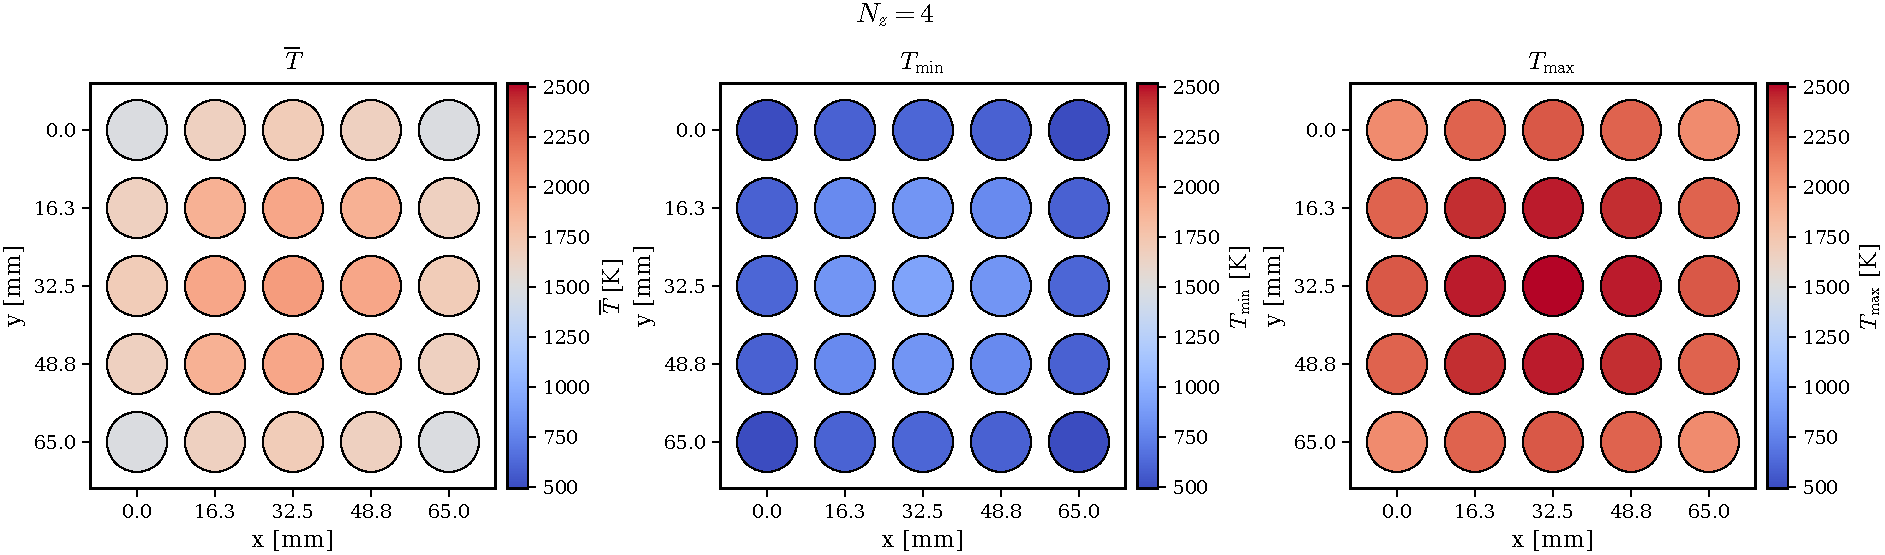
\includegraphics[width=0.8\linewidth]{PICTURES/c5couplage/T1800/assembly_4.pdf}

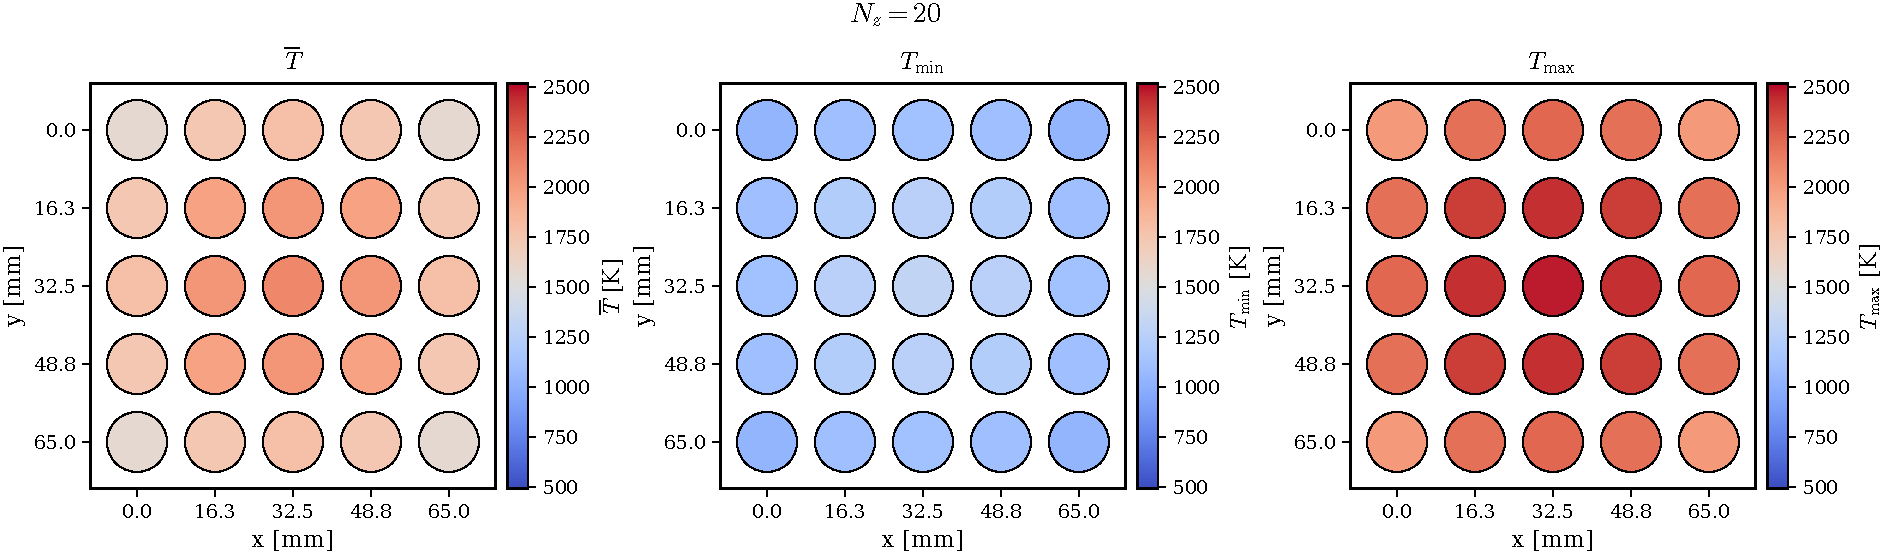
\includegraphics[width=0.8\linewidth]{PICTURES/c5couplage/T1800/assembly_20.pdf}

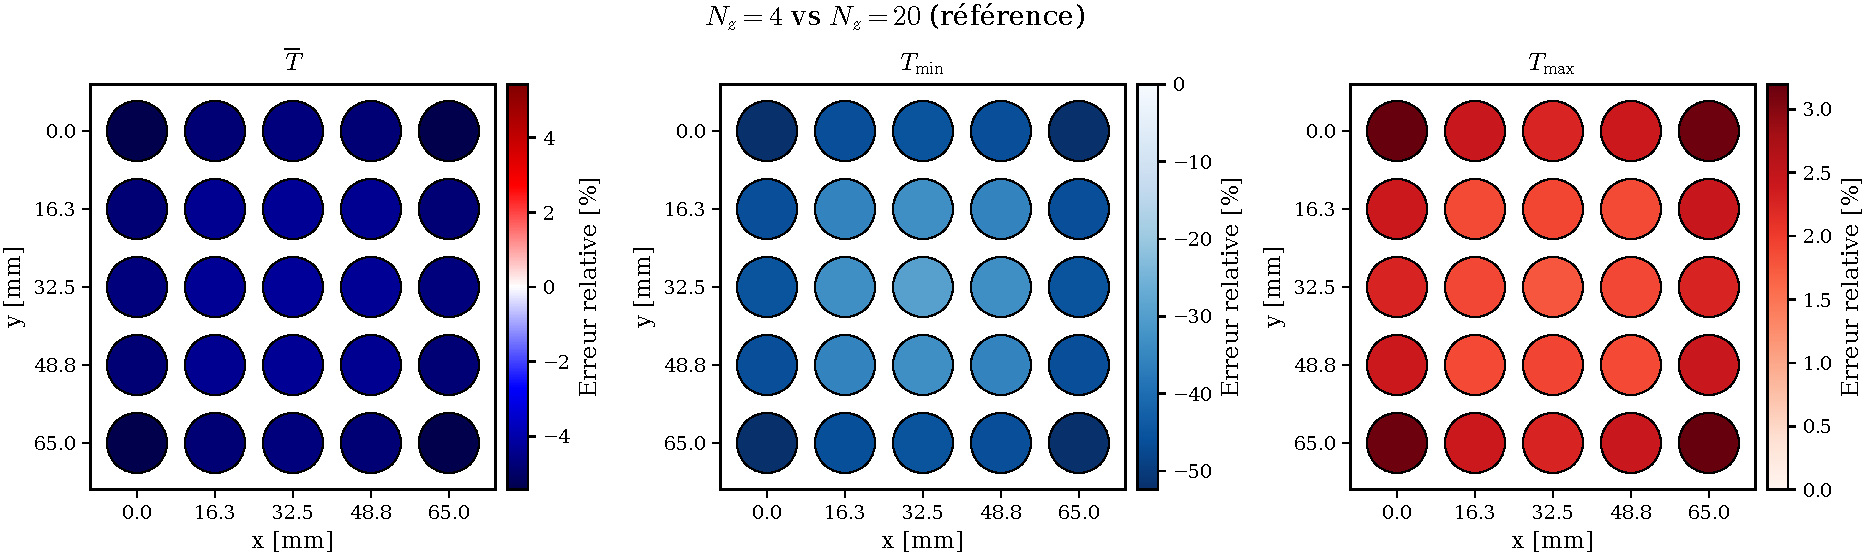
\includegraphics[width=0.8\linewidth]{PICTURES/c5couplage/T1800/assembly_diff_4_vs_20.pdf}
\caption{Champs de température pour le niveau de puissance le plus élevé : $N_z=4$ (haut), $N_z=20$ (milieu) et différence entre les deux champs (bas).}
\label{fig:temperature45MW}
\end{figure}

\begin{figure}[H]
\centering
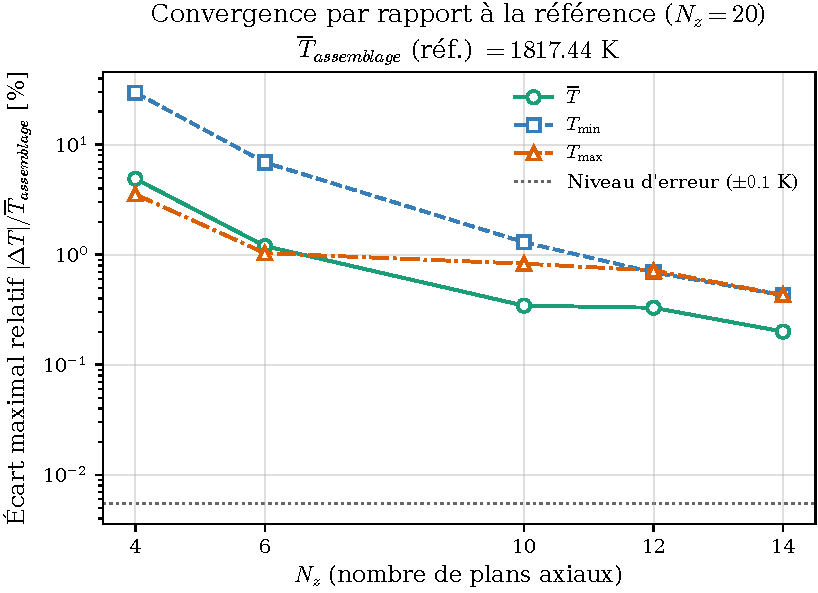
\includegraphics[width=0.7\linewidth]{PICTURES/c5couplage/T1800/convergence_relative_vs_20.pdf}
\caption{Écart relatif des températures minimale, maximale et moyenne en fonction de $N_z$, par rapport à la référence $N_z=20$, pour le niveau de puissance le plus élevé.}
\label{fig:convergence45MW}
\end{figure}

La Figure~\ref{fig:convergence45MW} montre que l'influence de la discrétisation axiale change qualitativement de régime pour ce niveau de puissance. La convergence vers la solution de référence est toujours observée, mais les écarts aux faibles valeurs de $N_z$ atteignent désormais des amplitudes d'un autre ordre : $T_{\max}$ est surestimée jusqu'à $3\,\%$, tandis que $T_{\min}$ et $\overline{T}$ sont sous-estimées respectivement jusqu'à $52\,\%$ et $5\,\%$.

\begin{table}[H]
\centering
\caption{Écarts relatifs maximaux observés par rapport à la référence $N_z=20$ pour $\overline{T}=1817~\mathrm{K}$.}
\label{tab:ecarts_discretisation_axiale_dernier}
\begin{tabular}{lcc}
\hline
Grandeur & Sens de l'écart & Écart maximal \\
\hline
$T_{\max}$ & Surestimation & $+3\,\%$ \\
$T_{\min}$ & Sous-estimation & $-52\,\%$ \\
$\overline{T}$ & Sous-estimation & $-5\,\%$ \\
\hline
\end{tabular}
\end{table}

Ces résultats constituent une rupture nette par rapport aux deux niveaux de puissance précédents : alors que la température moyenne n'était affectée que de $0{,}5\,\%$ au plus, son écart atteint ici $5\,\%$, et celui sur $T_{\min}$ dépasse $50\,\%$. La discrétisation grossière ne produit donc pas une erreur uniforme sur le champ thermique : elle affecte de manière disproportionnée les régions froides et les grandeurs qui leur sont attachées.

Ce changement de régime résulte de l'augmentation simultanée du niveau de température et des gradients thermiques. À cette puissance, les écarts de température entre régions de l'assemblage deviennent considérables ; une sous-géométrie couvrant une portion axiale étendue regroupe alors des zones dont les températures diffèrent fortement, et l'écart $\overline{T^4}-\overline{T}^{\,4}$ de l'inégalité~\eqref{eq:jensen} croît d'autant. La température homogénéisée cesse d'être représentative des conditions locales, et l'erreur commise sur le bilan radiatif devient suffisamment importante pour modifier le champ thermique lui-même.

Cette propagation explique également que la température moyenne soit désormais affectée de manière non négligeable. Un écart de $5\,\%$ ne peut plus relever d'une perturbation locale s'annulant par compensation spatiale : il traduit une modification du bilan radiatif suffisamment significative pour déplacer l'équilibre thermique global de l'assemblage.

La température maximale reste comme pour les autres cas moins sensible, son écart ne passant que de $0{,}9\,\%$ à $3\,\%$.

Comme pour les cas précédents, la convergence du solveur ne saurait expliquer ces écarts : avec une température moyenne stabilisée à $0{,}1~\mathrm{K}$ près, l'incertitude relative associée est de l'ordre de
\begin{equation}
\frac{0{,}1}{1817}
\approx 5{,}5\times10^{-5},
\end{equation}
soit près de trois ordres de grandeur en dessous des écarts mesurés. Ceux-ci sont donc bien attribuables à la représentation axiale des échanges radiatifs.

Ce dernier cas met ainsi en évidence une limite intrinsèque du modèle de discrétisation axiale. Alors que des valeurs modérées de $N_z$ suffisent aux deux premiers niveaux de puissance, elles deviennent inacceptables lorsque le niveau de température et les gradients thermiques augmentent fortement : une erreur de $52\,\%$ sur $T_{\min}$ et de $5\,\%$ sur la température moyenne signifie qu'une discrétisation trop grossière ne fausse plus seulement les valeurs locales, mais le bilan thermique global de l'assemblage. Le choix de $N_z$ ne peut donc pas être fixé sur la seule base d'un cas à puissance modérée ; il doit être établi en tenant compte du niveau de température et de l'intensité des gradients attendus sur l'ensemble des configurations étudiées.

Cette analyse confirme que le raffinement axial est un paramètre déterminant pour la représentativité du calcul radiatif. Aux niveaux de puissance les plus élevés, une discrétisation suffisamment fine est indispensable pour limiter l'erreur associée à l'hypothèse de radiosité unfirome et température constance par surface et garantir une précision acceptable sur l'ensemble du champ thermique, en particulier dans les régions les plus froides.

\subsection{Étude de l'écart entre le point chaud et la température moyenne}

Le Tableau~\ref{tab:tmoy_tmax} rassemble, pour les différents niveaux de puissance étudiés, la température moyenne de l'assemblage $T_{\mathrm{moy}}$ et la température de point chaud du système. Pour des raisons de compromis entre temps de calcul et convergence, une découpe en 14 sections axiales a été choisie. Le biais lié à l'hypothèse de radiosité uniforme est alors de l'ordre du pour mille. Cette étude correspond au maximum des températures maximales relevées sur l'ensemble des crayons de l'assemblage, $T_{\mathrm{max}} = \max_i \left( T_{\mathrm{max},i} \right)$, qui coïncide avec la température maximale du crayon central, celui-ci étant le plus exposé thermiquement du fait de sa position au cœur de l'assemblage. On observe que l'écart entre $T_{\mathrm{max}}$ et $T_{\mathrm{moy}}$ croît avec le niveau de puissance déposée, aussi bien en valeur absolue qu'en proportion de la température moyenne.

L'intérêt de ce résultat ne réside pas uniquement dans ces valeurs prises isolément, mais dans la démarche qu'elles illustrent : la capacité à quantifier, à partir d'une simulation CFD 3D convergée, l'écart entre température moyenne et température de point chaud pour une configuration donnée. Une telle relation, une fois établie sur un nombre suffisant de cas, ouvrirait la voie à l'estimation de la température de point chaud d'un système à partir de sa seule température moyenne, cette dernière étant directement accessible par des modèles à zones plus simples et bien moins coûteux en temps de calcul que la simulation CFD 3D complète.

Il convient toutefois de discuter dans quelle mesure ce résultat dépend du profil de puissance retenu. Le profil axial en cosinus utilisé dans cette étude, représentatif de la distribution de puissance neutronique le long d'un crayon, concentre le dépôt de puissance au centre du domaine actif et atténue les effets de bord en haut et en bas du crayon. Ce choix exacerbe mécaniquement l'écart $T_{\mathrm{max}} - T_{\mathrm{moy}}$ par rapport à un profil plat, mais il correspond à des situations physiquement réalistes en réacteur. La position du point chaud (crayon central, cote axiale médiane) ne varie pas avec le niveau de puissance étudié, ce qui conforte la robustesse de la corrélation établie.

La modélisation de l'écart relatif en fonction de la température moyenne, présentée en Figure~\ref{fig:hotspot}, s'ajuste par une loi de la forme
\begin{equation}
\frac{T_{\mathrm{max}} - T_{\mathrm{moy}}}{T_{\mathrm{moy}}} = A + C \exp\left(-\frac{T_{\mathrm{moy}}}{\tau}\right),
\end{equation}
avec $A$, $C$ et $\tau$ des paramètres ajustés sur les données. Cette expression traduit la saturation progressive de l'écart relatif aux températures élevées, où le transfert radiatif tend à homogénéiser le champ thermique. La faisabilité d'une telle démarche sur un assemblage $5\times5$, bien que simplifié par rapport à une géométrie de cœur réel, démontre le potentiel de cette approche pour des configurations industrielles plus représentatives.

\begin{table}[H]
\centering
\begin{tabular}{cccc}
\toprule
Puissance volumique~[$\mathrm{MW/m^3}$] & $T_{\mathrm{moy}}$~[K] & $T_{\mathrm{max}}$~[K] & Écart relatif $\frac{T_{\mathrm{max}} - T_{\mathrm{moy}}}{T_{\mathrm{moy}}}$ \\
\midrule
$3$  & $925{,}2$ & $1127$ & $21{,}81\,\%$ \\
$4$  & $981{,}5$ & $1211$ & $23{,}38\,\%$ \\
$5$  & $1028$    & $1280$ & $24{,}51\,\%$ \\
$10$ & $1215$    & $1560$ & $28{,}40\,\%$ \\
$20$ & $1453$    & $1915$ & $31{,}80\,\%$ \\
$30$ & $1621$    & $2170$ & $33{,}87\,\%$ \\
$40$ & $1756$    & $2376$ & $35{,}31\,\%$ \\
$45$ & $1817$    & $2475$ & $36{,}21\,\%$ \\
\bottomrule
\end{tabular}
\caption{Température moyenne de l'assemblage et température de point chaud (crayon central) pour les niveaux de puissance étudiés.}
\label{tab:tmoy_tmax}
\end{table}

\begin{figure}[H]
\centering
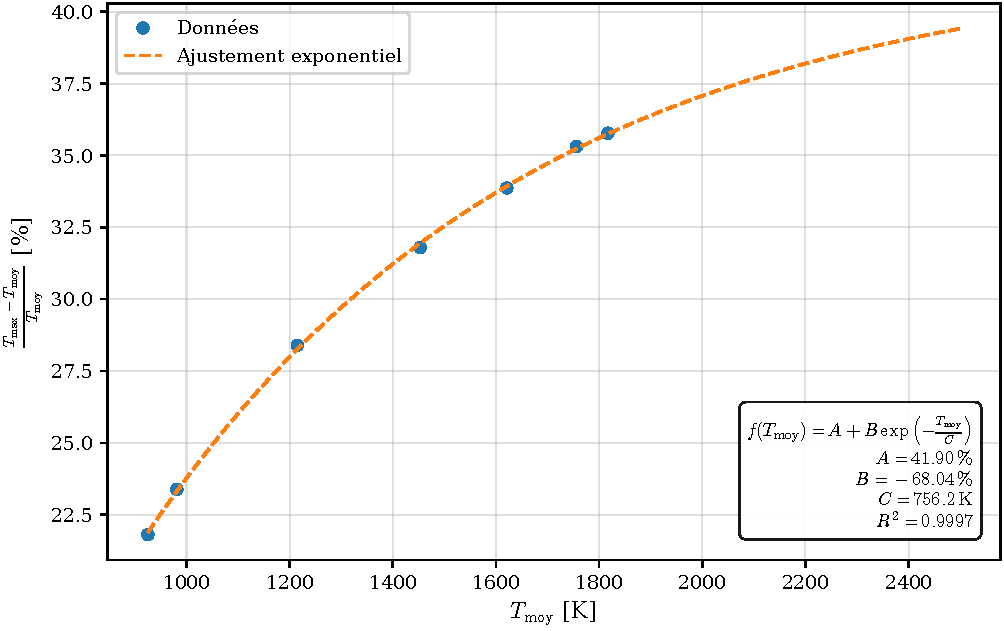
\includegraphics[width=0.7\linewidth]{PICTURES/c5couplage/hot_spot.pdf}
\caption{Modélisation de l'écart de la température maximale par rapport à la température moyenne.}
\label{fig:hotspot}
\end{figure}


\subsection{Conclusion}

Ce chapitre a permis de démontrer la faisabilité d'une étude CFD 3D couplée conduction--rayonnement sur une géométrie représentative d'un assemblage de crayons combustible en réseau $5\times5$. À travers une campagne de simulations paramétriques, trois résultats principaux ont été mis en évidence.

\textbf{Premièrement}, la discrétisation axiale des surfaces dans le calcul radiatif constitue un paramètre déterminant pour la précision du bilan thermique global. L'inégalité de Jensen, appliquée à la loi de Stefan--Boltzmann, fournit le cadre théorique permettant de comprendre pourquoi l'homogénéisation de la température par sous-géométrie sous-estime systématiquement la puissance radiative émise dès qu'un gradient thermique est présent. Cette sous-estimation se propage à travers le réseau d'échanges radiatifs et affecte de manière significative les températures du système et mérite d'être étudié en profondeur.

\textbf{Deuxièmement}, l'amplitude de l'erreur induite par une discrétisation grossière croît fortement avec le niveau de puissance déposée. Aux faibles puissances ($3$ et $4~\mathrm{MW/m^3}$), un nombre de tranches axiales $N_z = 14$ suffit à garantir des écarts relatifs inférieurs au pour cent sur la température moyenne et aux températures extrêmes. En revanche, à forte puissance ($45~\mathrm{MW/m^3}$), une discrétisation identique conduit à des écarts de $52\,\%$ sur $T_{\min}$ et de $5\,\%$ sur $\overline{T}$, traduisant une modification du bilan thermique global de l'assemblage. Le choix de $N_z$ ne peut donc pas être fixé une fois pour toutes : il doit être adapté au régime thermique considéré.

\textbf{Troisièmement}, la simulation CFD 3D offre la possibilité d'établir une corrélation entre température moyenne et température de point chaud. L'écart relatif $T_{\mathrm{max}} - T_{\mathrm{moy}}$ croît avec la puissance déposée et peut être modélisé par une loi de saturation, ouvrant la voie à une estimation de la température de point chaud à partir de modèles à zones plus simples et moins coûteux. La position du point chaud (crayon central, cote axiale médiane) se révèle invariante avec le niveau de puissance, ce qui renforce la robustesse de cette approche.

Ces travaux ouvrent plusieurs perspectives. L'extension de cette démarche à des géométries industrielles plus représentatives, incluant notamment des assemblages de plus grande taille et des profils de puissance plus complexes, permettrait de valider la généralité de la corrélation établie. Par ailleurs, l'étude de l'influence conjointe des discrétisations angulaire et axiale sur la précision du calcul radiatif constituerait un prolongement naturel de cette analyse. Enfin, l'intégration de cette corrélation dans un modèle à zones amélioré permettrait de combiner la rapidité de calcul des approches simplifiées avec la précision des simulations CFD 3D sur les grandeurs critiques de sûreté.
